
%What is eels?
%Sample experimental setup
%Sample spectra
%Signal types
%usages
%pros, cons/ STEM TEM
\setcitestyle{numbers,open={[},close={]}}

 


Many of the results from EELS have non-intuitive interpretations, particularly in the case of ELNES which relies largely on qualitative comparisons between measured and database spectra.  Consequently, new materials and situations require a degree of theoretical support to analyze novel results.  This support often comes from ab initio calculations, amongst others density functional theory (DFT).  This section will describe the basis of DFT and its various implementations, as well as discuss the peculiarities of simulating lithium materials.

\subsection{Background}
DFT is an ab initio method that requires only atomic positions as input and is independent of experimental support.  By solving a modified version of the Schrodinger equation, it is possible to obtain the ground state energy of the system, and from there determine a range of other properties, including EELS spectra. This almost direct treatment of quantum mechanics make DFT one of the most accurate techniques, however, the quadratic to cubic scaling of the method, limit its applicability to small scale systems, Fig \ref{scaling}.  DFT's success and flexibility have resulted in the development of a large number (90+) of codes, both open source and commercial, and its place in a wide array of fields \cite{DFT_codes}.  

\begin{figure}
	\centering
	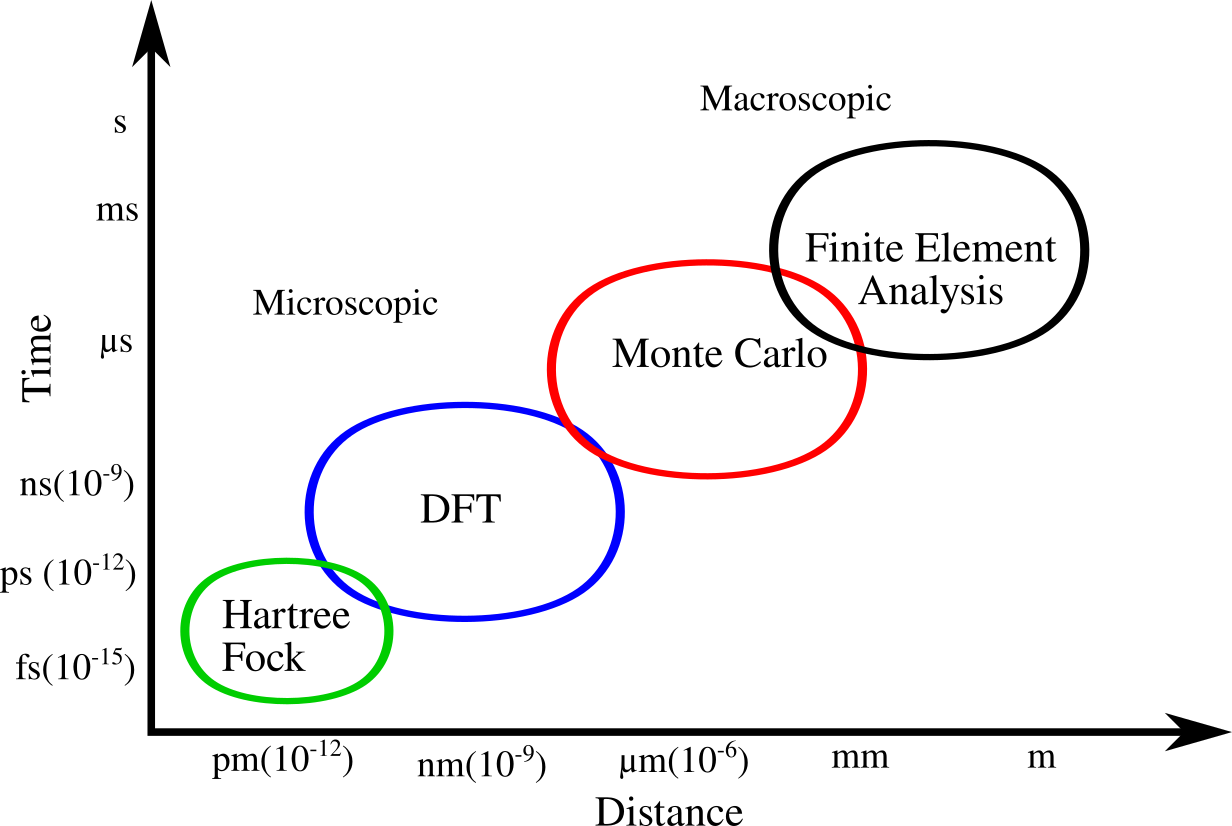
\includegraphics[scale=0.3]{method_scaling.png}
	\caption{Various methods available to compute material properties and their corresponding regions of use. }
	\label{scaling}
\end{figure}


\subsection{Formulation}

DFT is centred  on solving the many bodied  Schrodinger equation \cite{sholl_density_2009}.  The aim is to obtain a solution for $\psi$ from which observable properties can be calculated:  

\begin{equation}
	\frac{-\hbar^2}{2} \sum_{i}^{N} \frac{\nabla^2 \psi_i}{m_i} + \sum_{i}^{N} V(\textbf{r}_i) \psi_i = E \psi
\end{equation}

In this case, we will consider the non-relativistic, spin independent, time independent case, although more in-depth derivations can be found elsewhere \cite{tddft}.  We will now apply the Born Oppenheimer approximation which assumes that the nuclei can be separated from the electrons and will act classically. The validity of this assumption stems from the fact that nuclei are a  over 1000 times more massive than electrons \cite{graff_direct_1980}.  The Born Oppenheimer approximation allows us to only solve for the $\psi$ of electrons:

\begin{equation}
	\bigg[\frac{-\hbar^2}{2m_e}\sum_{i}^{N} \nabla^2 +\sum_{i}^{N} V(\textbf{r}_i) + \sum_{i}^{N}\sum_{j <i}U(\textbf{r}_i,\textbf{r}_j) \bigg] \psi_i(\textbf{r}_i) = E \psi_i
\end{equation}

Where $m_e$ is the mass of an electron, $N$ is the number of electrons, and $\textbf{r}_i$ is a position vector. The terms inside the square brackets are collectively know as the Hamiltonian and are respectively: the kinetic energy of all the electrons, the Coulomb interaction between the electrons and the nuclei, and the electron-electron Coulomb interaction  \cite{sholl_density_2009}. At this point, these equations are still too unwieldy to solve, depending on 3N variables (the position coordinates of each wavefunction), not to mention the many body problem lurking inside the double sum.  Facing this conundrum, we take advantage of the Hohenberg-Kohn Theorems which postulates \cite{hohenberg_inhomogeneous_1964}:
\begin{itemize}
	\item  The ground state \textit{energy} of the system is a unique functional of the ground state \textit{electron density}.
	\item The electron density that minimizes the overall energy corresponds to the real ground state density.  
\end{itemize}

By changing the variables being solved for to the \textit{density} and not wavefunctions, we can simplify the problem down to only three variables: the three coordinates of the density field.  The Hohenberg-Kohn theorems indicate that we can make everything a functional of electron density and that any density other than the groundstate will result in a higher energy in the system \cite{parr_density_1983}.  We now define the term functional, as an object that acts like a function, except takes other functions as input instead of variables, eg:

\begin{equation}
F[f(x)] = f(x)^2 
\end{equation}

 In the case at hand, the relevant functional is the energy which is a functional of the density: $E[n(\textbf{r})]$.  Using the Hohenberg-Kohn theorems, we can begin working towards a more manageable equation for energy as a functional of density by further breaking down the potentials: 
\begin{equation}
-\frac{\hbar}{2m_e} \sum_{i} \int \psi_i^* \nabla^2\psi_id^3r + \int V(\textbf{r})n(\textbf{r})d^3r + \frac{e^2}{2} \int \int \frac{n(\textbf{r})n(\textbf{r}')}{|r-r'|}d^3r d^3r' + E_{\mathrm{nuclei}} + E_{\mathrm{XC}} = E[n(\textbf{r})]
\end{equation}

Where, the second term is the energy from the electron density-nuclei interaction with $V(\textbf{r})$ is the electric field created by the nuclei; the third term is the electron density-electron density Coulomb interaction and $E_{\mathrm{nuclei}}$ is the contribution from nucleus-nucleus interaction.  The final term, $E_{XC}$ is the exchange and correlation term and is where all of the quantum features of the electrons have been grouped; the price to pay for substituting in density. This equation cannot be directly solved from first principles by itself as we need some way to obtain the electron density.  On this front we introduce the Kohn -Sham equations which assume that we can decouple all of the electrons into single particle equations: 

\begin{equation}
    \bigg[T_i + V(\textbf{r}) + V_{\mathrm{H}}(\textbf{r}) + V_{\mathrm{XC}}(\textbf{r})\bigg] \phi_i(\textbf{r}) = \epsilon_i \phi_i(\textbf{r})
    \label{ks_eq}
\end{equation}

Where $\phi_i$ and $\epsilon_i$ are the Kohn sham wavefunctions and eigenvalues respectively and $V_H$ is the Hartree potential or: 
\begin{equation}
    V_\mathrm{H} = e^2 \int \frac{n(\textbf{r'})}{|\textbf{r}-\textbf{r'}|}d^3r'
\end{equation}
Which represents the interaction of the electron in question (the one at $\textbf{r}$, not $\textbf{r'}$) and all the electrons in the sample.  This results in some interaction between the electron and itself, a term that must be corrected for in the $V_{XC}$ term.  The Kohn-Sham equations can  be readily solved, but require the density to calculate the Hartree potential.  The density is in turn given from the wavefunctions: 
\begin{equation}
	n_{\mathrm{KS}}(\textbf{r}) = 2 \sum_{i} \phi_i^*\phi_i
	\label{KS_density}
\end{equation}
Where the two is to account for electron spin.  As the density is needed to calculate the wavefunctions and vice versa, a self consistent approach must be taken in order to obtain a valid result:  

\begin{enumerate}
	\item Assume a starting density
	\item Use the initial density to calculate the Hartree potential and use it to solve the Kohn-Sham equations for the wavefunctions
	\item Calculate a new density using Eqn. \ref{KS_density}.
	\item Compare the new density to the initial, update the initial density. 
	\item Repeat steps 2-4 until the density converges and the energy is minimized. This density then represents the groundstate for the system.
\end{enumerate}

This method is the starting point for DFT calculations, from here there are a number of different variations with regards how to go about these steps.  Amongst others, the treatment of the exchange-correlation potential and choice of basis for the wavefunctions is what separates the methods.  


\subsubsection{Exchange-Correlation Potential}
The exchange-correlation potential was introduced above, but not defined.  That is because there no easily solvable form for this term as it must collect all of the unknown features not accounted for in the rest of the Kohn-Sham equations, including electron's being indistinguishable, the self interaction term, etc.   There have been a number of proposed potentials, many designed for specific situations the most common of which will be discussed here.  Like the other potentials in the Kohn-Sham equations, the XC potential is defined as a functional of density.  The various potentials vary according to accuracy and computational cost.  The first attempt, originally proposed by Kohn and Sham in 1965 was the local density approximation (LDA) in which the XC potential depends only on the density \cite{tao_climbing_2003, ks_1965}: 

\begin{equation}
	E_{\mathrm{XC}}[n(\textbf{r})] = \int  n(\textbf{r}) \epsilon_{\mathrm{XC}}[n(\textbf{r})] d^3r
\end{equation}

LDA is exact in the case of a free electron gas and has obtained good success when applied to metallic solids.  By considering the gradient of the density as well, a more involved potential is obtained, called the generalized gradient approximation (GGA) \cite{tao_climbing_2003,perdew_wang} : 


\begin{equation}
E_{\mathrm{XC}}[n(\textbf{r})] = \int  n(\textbf{r}) \epsilon_{\mathrm{XC}}[n(\textbf{r}), \nabla n[\textbf{r}]] d^3r
\end{equation}


Other parameters can also be taken into consideration, such as the potential energy (meta GGA) or empirical factors (hybrid functionals) \cite{tao_climbing_2003, bj_pot}.  Depending on the desired property and available computing power, an appropriate functional should be chosen for each case.


\subsubsection{Basis Sets}
A second defining feature for DFT is the choice of basis set for the wavefunctions, $\phi_i$, and a number of options have become prevalent in the available programs.  These are divided into two distinct types, localized and periodic \cite{sholl_density_2009}.  Localized basis sets rely on using orthogonal functions that decay rapidly away from the origin \cite{sholl_density_2009}.  An example is Gaussian peaks, as is used in the Gaussian16 software package \cite{g16}.  The very localized basis set is useful for handling single, isolated molecules, and as such is ideally suited applications in quantum chemistry and biology. Poor scaling with electron number (typically N$^3$ or worse) limits the maximal size of system that can be studied \cite{mohr_linear_2018}.  In materials science, a typical system of interest is a bulk material and thus unsuitable for this type of approach.  To handle these cases, periodic basis sets are used, by defining a unit cell and repeating it infinitely in all directions.  The solution to the Schr\"odinger equation under these periodic boundary conditions is given by Bloch waves, defined as \cite{griffiths}:

\begin{equation}
	\psi = u(\textbf{r}) e^{i\cdot \textbf{k}}
\end{equation}

Consequently, a natural basis choice for periodic boundary situations are plane waves, which are used in a number of DFT packages including VASP, Quantum Espresso, and Wien2k \cite{qe,vasp,wien2k}.  The periodic boundary method allows for accurate calculation of in infinitely samples representative of bulk materials.  Computation limits still apply to the size of the unit cell, typically limited to at most a few hundred atoms \cite{mohr_linear_2018}.  This effect renders features such as defects and grain boundaries highly computationally expensive as they must be contained in a cell large enough to isolate them from their images in adjacent cells. 
As large numbers of plane waves would be required to handle the fine features in the electron density close to nuclei, often an augmented plane wave (APW) technique is used.  APW lowers the computational cost by dividing the unit cell into two regions: interstitial space and atomic basins (sometimes referred to as muffin tins), illustrated in Fig \ref{MT} \cite{wien2k}. 
\begin{figure}
	\centering
	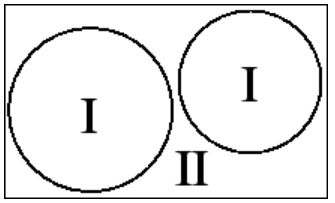
\includegraphics[scale=0.5]{muffin_tins.png}
	\caption{The two regions in an APW approach.  (I) Atomic Basins modelled with Psudopotentials or atomic orbitals and (II) interstitial space modelled with a plane wave basis set \cite{wien2k}. }
	\label{MT}   
\end{figure}

The ability to divide electrons into two groups is due to the fact that the core electrons surrounding each atom are largely unaffected by their local environment as they are screened by the outer shells \cite{wien2k}. The choice of which basis set is used inside the muffin tins provides further options between DFT codes.  One option is pseudopotentials, which are pre-generated densities for each element, which can be varied to match the plane waves at the boundary \cite{singh_planewaves_2006}.  The pseudopotential method is used in a number of codes, amongst others, VASP and Quantum Espresso \cite{vasp,qe}.  Alternatively, spherical harmonics corresponding to the atomic orbitals can be used for increased accuracy \cite{griffiths}. This type of DFT is referred to as all-electron or full potential, as every electron is represented in the basis set, unlike the pseudopotential method where many are absorbed into the pre-calculated PP \cite{wien2k}. Fitting for all of the electrons in the sample comes at a computational cost, yet allows for more accurate analysis of properties dependent on core states, such as ELNES spectra in EELS.   
 
 A flowchart demonstrating the various properties of some common DFT codes is presented in Fig \ref{dft-flowchart}.  The DFT code used primarily in this work is Wien2k.

\begin{figure}
	\centering
	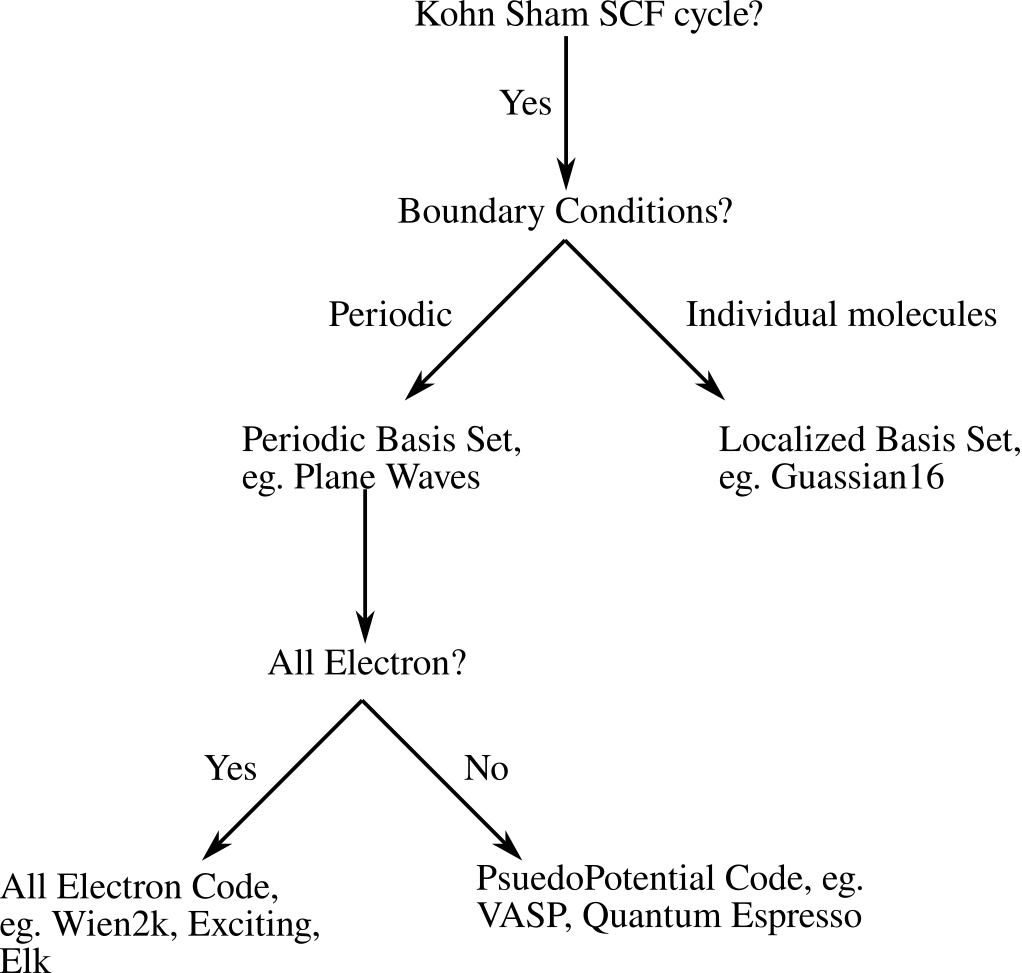
\includegraphics[scale=0.3]{DFT_flowchart.png}
	\caption{Flowchart depicting the various choices of basis set available to DFT codes.}
	\label{dft-flowchart}
\end{figure}


\subsection{WIEN2k}
WIEN2k is an all electron code that uses a linearized augmented plane wave (LAPW) formulation, combining plane waves with spherical harmonics as in Fig \ref{MT} \cite{wien2k}.   In WIEN2k's standard formalism, the basis sets for the Kohn-Sham wavefunctions can be represented as: 

\begin{equation}
	\phi_{\mathrm{k}_n} = 
	\begin{cases}
	\Sigma_{lm} [A_{lm,\textbf{k}_n}u_l(r,E_l) + B_{lm,\textbf{k}_n}\dot{u}_l(r,E_l)]Y_{lm}(\hat{\textbf{r}}) & r \leq r_{\mathrm{RMT}} \\
	\frac{1}{\sqrt{\omega}}e^{i\textbf{k}_n \cdot \textbf{r}} & r> r_{\mathrm{RMT}} \\
	\end{cases}
\end{equation}

Where $Y_{lm}(\hat{\textbf{r}})$ are the spherical harmonics and $u_l(r,E_l)$ are the solutions to the radial Schr\"odinger equation.  The coefficients $A_{lm,\textbf{k}_n}$ and $B_{lm,\textbf{k}_n}$ are set so as to match the value and slope of the plane waves at the boundary \cite{wien2k}.  The use of an all electron code is essential for computing EELS accurately as it allows a more flexible treatment of core electrons not granted in pseudopotential codes. 
 


\subsection{Quantum Theory of Atoms in Molecules} \label{bader-theory}
Before continuing to the application of DFT to EELS, we will briefly discuss a more direct application of DFT; defining atoms and bonds from the electron density. Initial work on this front was performed by Bader \cite{bader}. The electron density can be divided into regions, with each atomic basin  delimited by surfaces satisfying \cite{bader_quantum_1991}: 


\begin{equation}
\nabla \rho(\textbf{r}) \cdot \textbf{n}(\textbf{r}) = 0   \hspace{1cm} \forall\textbf{r} \in S(\Omega,\textbf{r})
\label{basin_surface}
\end{equation}

That is, surfaces with no flux of electron density through them and can be pictured as a ``valleys" in the electron density ``landscape," see Fig \ref{topo_plot}. In order to  calculate the location of these surfaces, critical points in the density field are located, defined when $\nabla \rho(\textbf{r})=0$, and always satisfy Eq. \ref{basin_surface}.  With the exception of critical points at maximas in $\rho(\textbf{r})$ which are located at nuclei, all of the critical points lie on interatomic surfaces \cite{critic2}. The nature of the critical points can then be evaluated (minima, first or second order saddle point), and the location of bonds which are centred on first order saddle point critical points, can be determined \cite{critic2}.  The bonds can then be characterized to provide first principles chemical bonding analysis for quantum chemistry \cite{fugel_variety_2018}.  

\begin{figure}
	\centering
	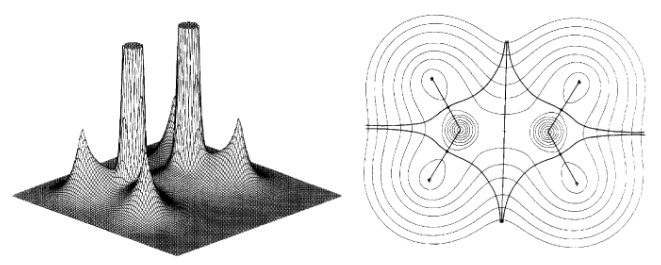
\includegraphics[scale=0.5]{bader_topo_plot}
	\caption{Density plot (left) and identification of atomic basin (right) in diborane atomic From Bader \cite{bader}.}
	\label{topo_plot}
\end{figure}


\subsection{Lithium in DFT}
As in experiment, lithium's low atomic number requires a number of special treatments  in DFT.  These are largely due to loosely bound electrons with large orbitals resulting from lithium's small nuclear charge.  As a result, even the 1s level electrons in lithium can have orbitals extending well past 2.5 Bohr from the nuclei, far further than in heavier elements, see Fig \ref{orbital_size} \cite{mauchamp_ab_2006}.  This results in a number of issues. Firstly, it is difficult and sometimes impossible to set the atomic sphere radii large enough to contain all these 1s core electrons.  As atomic spheres cannot overlap, they are typically limited to $\sim$ 2.0 Bohr. Depending on the compound, the sphere size can be further constrained as all the spheres must be roughly the same size (within 30\%) \cite{wien2k}.  If the sphere sizes are too varied, convergence time and accuracy can deteriorate dramatically.  The alternative to large sphere size is to allow a degree ($\sim$0.5\%)of core leakage into the calculation \cite{wien2k}.  The downside to allowing leakage is that it may result in non physical effects at later stages in the calculation, or result in the appearance of ``ghostbands" in the calculation \cite{wien2k}.

\begin{figure}
	\centering
	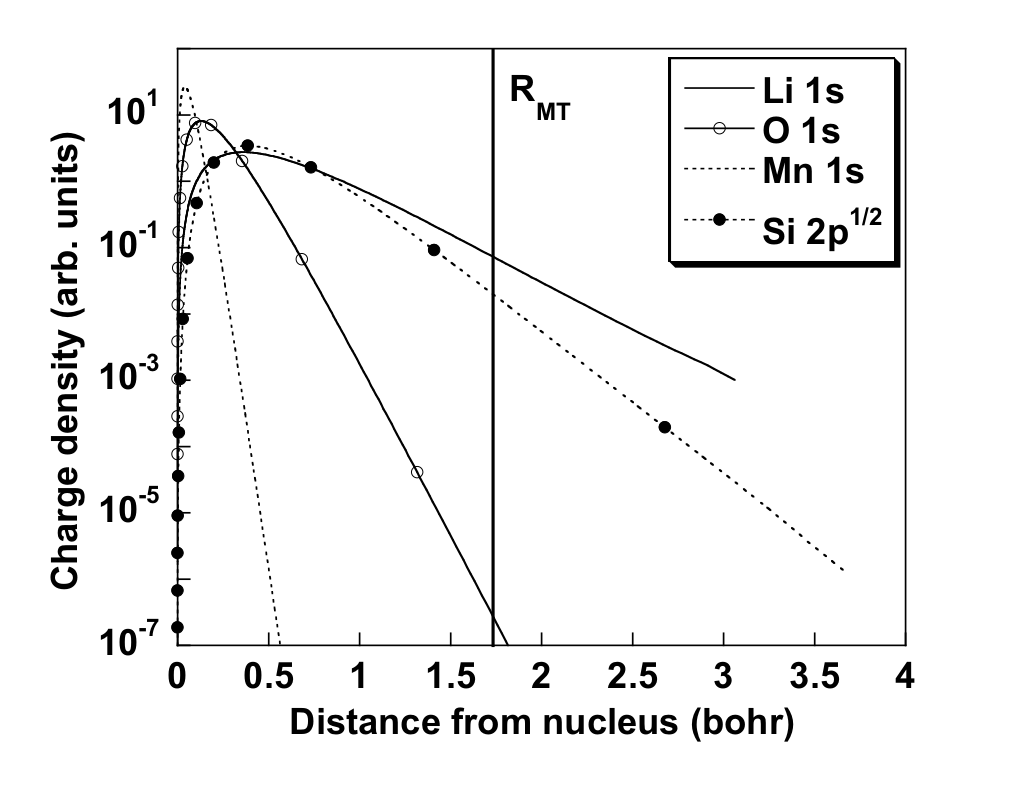
\includegraphics[scale=0.3]{atomic_orbital_size}
	\caption{Orbital charge densities as a function of distance from nucleus, demonstrating the varying degrees of localization.  From Mauchamp et al \cite{mauchamp_ab_2006}}
	\label{orbital_size}
\end{figure}



